\section{Application to the COVID-19 outbreak}

The model described in Section~\ref{sec:model} is tuned here to fit at best the dataset from Lombardy shown in Figure~\ref{fig:data_lombardy}. Since the data available show just the leading curve of the outbreak, only parameters $\beta$, $\braket{k}$, $\delta$ and $\tau$ have to be tuned. Moreover, an additional parameter $t_0$ has been added to shift the distribution in time. The available dataset regards the \emph{total cases}, corresponding to the sum of infected (positively tested), recovered and deaths. This is not immediately comparable with the population classes in the model. Here it is identified as the sum of quarantined, recovered and deaths. Infected population is not included in the total number because it would correspond to the whole infected population being tested as positive, even the population not showing symptoms, highly probable in young population. Therefore the infected population correspond to the part of the population that has the virus but has not been tested, and all the positively tested population is immediately quarantined. The best fitting setup is shown in Figure~\ref{fig:data_vs_model_first_lombardy}. Parameters modifying the trailing edge of the infection is set to approximate values of the outbreak. Mortality is set to $2\%$, reinfection probability to $10^{-5}$ since yet no cases have been observed. Population is set to $10^7$, corresponding to Lombardy population.\\

\begin{figure}
\centering
  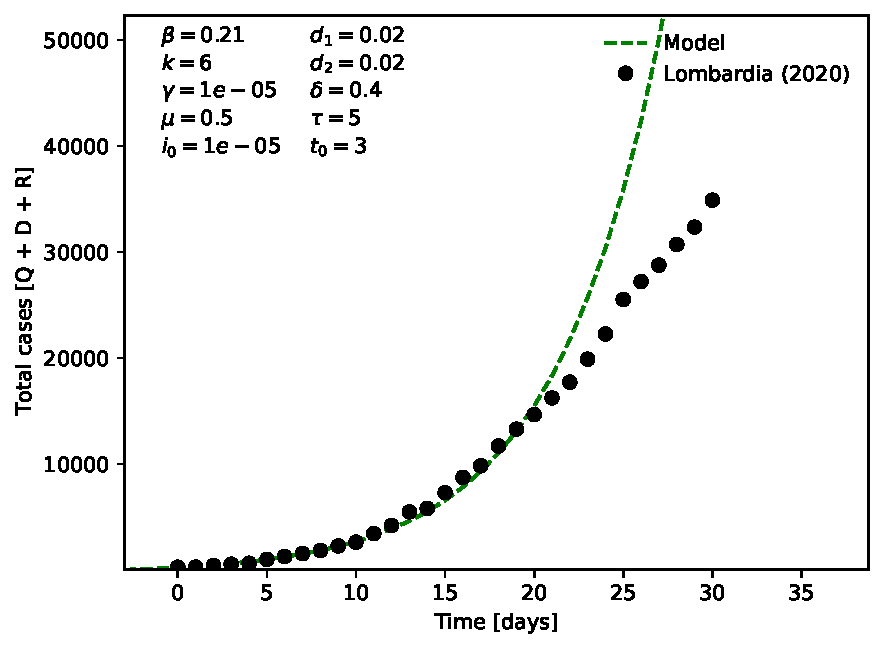
\includegraphics[width=0.4\textwidth]{imgs/Covid/DataVsModel_parameters_Lombardia_less_impacting.pdf}
  \caption{Best match of parameters to make the model described in Section~\ref{sec:model} fit with data il Lombardy.}
  \label{fig:data_vs_model_first_lombardy}
\end{figure}

As shown in Figure~\ref{fig:data_vs_model_first_lombardy} the model predicts an exponential growth until reaching a peak, that is not what is measured, since different slopes in the total cases curves are present. Possibly this is due to changing in the small-world conditions such as limitation to the social activity (mandatory closings of shops, cancellations of events, etc.), improvements of the sanitary checking and testing. This should cause a decrease of the slope, instead of an increase, caused, for example, by a longer incubation time. This hypothesis is quite encouraged by the dates on data when the change of slopes occur: around March 10th and 20th. On March 9th and 11th two special laws have been approved and applied, closing all shops, limitation of movements for citizens. On March 10th even a tighter regulation have been introduced: no movements among cities and mandatory closing of all the activities except for hospital, farmacies, hostera and corresponding chains. The corona virus' incubation time, although the recommended quarantine of fifteen days, it has a shorter incubation time before possible symptoms happen of less than a week. Therefore the effects of the actions affect the curve in few days.\\

The idea to adapt the model to the real world scenario, two improvements have been implemented:
\begin{itemize}
\item Scheduling of $\braket{k}$ parameter: this reflects the change in social activity in time.
\item Fluctuation of $\delta$ parameter: this reflects the fluctuation of the number of tests done per day.
\end{itemize}

No scheduling of $\delta$ parameter has been introduced. This implies that the fraction of the tested people is almost constant over time. This is encouraged by the constant testing strategy adopted in Lombardy and by the observed (almost) constant mortality rate  when normalised over the number of tests.\\



\subsection{Improvement of the model}
\label{ssec:impr_model}
Here the improvement applied to the model are described. The corrections of $\delta$ parameter are extrapolated from Figure~\ref{fig:tests_vs_time}. A functional model has been fitted to the data points and the corrections have been extracted as residual of the observed point with respect to the function. The function is consistent with the choice of constant $\delta$ since it approximately describe the data trend in Figure~\ref{fig:data_lombardy}.\\

\begin{figure}
\centering
  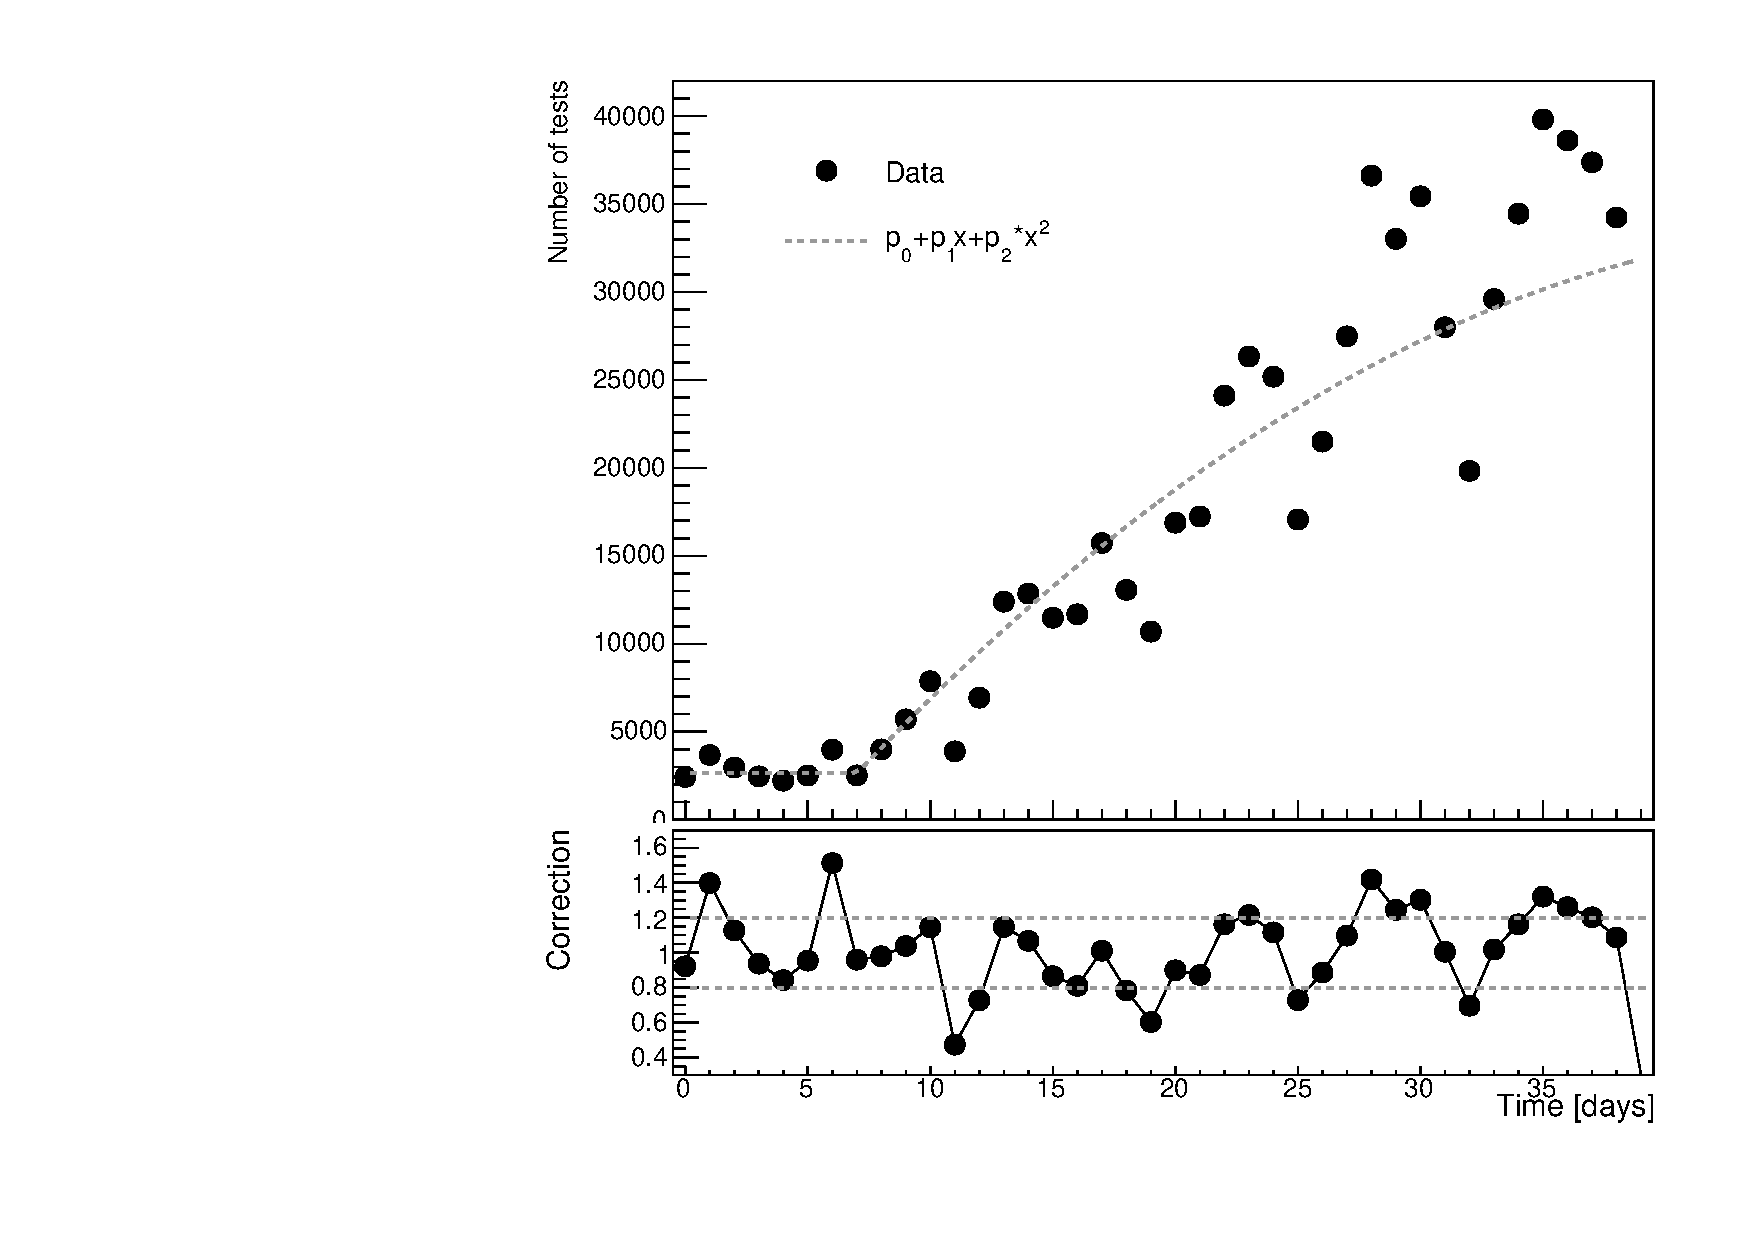
\includegraphics[width=0.4\textwidth]{imgs/Covid/TamponsCorrections.pdf}
  \caption{Numbers of tests performed against time in Italy. A constant plus a third degree polynominal has been fitted and corrections (plot below )have been extracted as difference of the measured point to the functional model.}
  \label{fig:tests_vs_time}
\end{figure}

This correction is introduce to describe the non-smooth behaviour of the curve. However, since this data are available national-wise, numbers for Lombardy may differ. This is take into account in the fit, described in Section~\ref{ssec:plf}. The $\braket{k}$ scheduling represents the limitation of the social interactions, from a freely-communicating system to isolation where an infected person may interact only with  few susceptible individual (family).\\

\begin{figure}
\centering
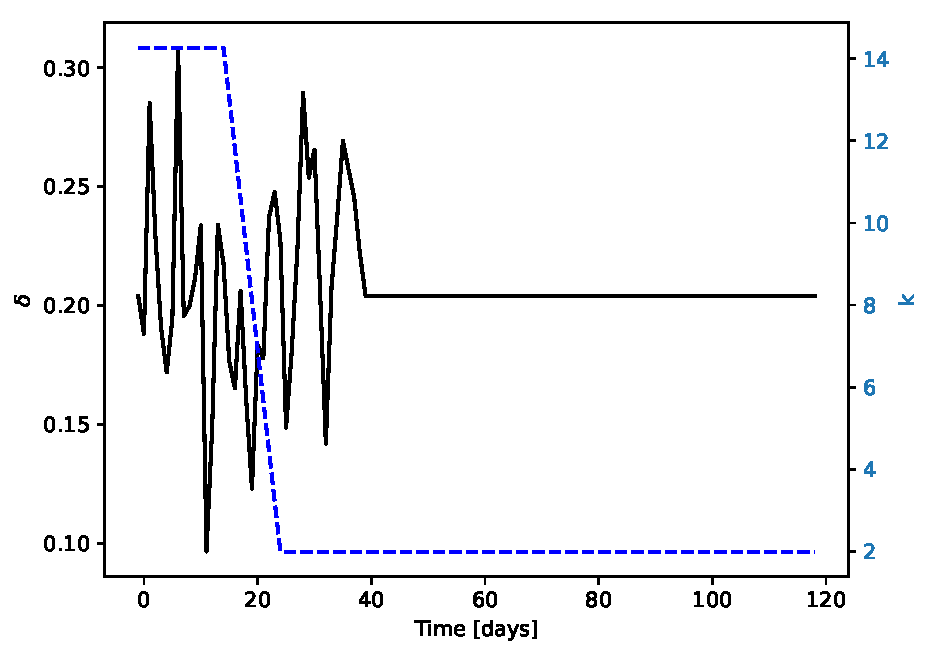
\includegraphics[width=0.4\textwidth]{imgs/Covid/Scheduling_regular.pdf} 
  \caption{Scheduling of $\delta$ and $\braket{k}$ parameters in time. The reference values of the parameters are set the same as in Figure~\ref{fig:data_vs_model_first_lombardy}.}
  \label{fig:scheduling}
\end{figure}

\begin{figure}
\centering
\subfloat[\label{fig:model_vs_time}]{ 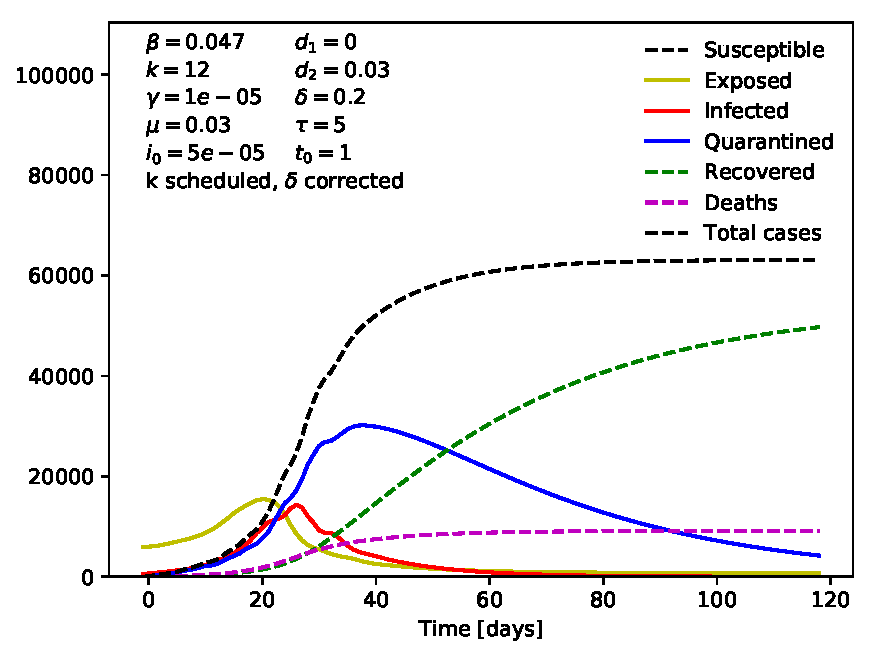
\includegraphics[width=0.4\textwidth]{imgs/Covid/Summary_parameters_Lombardia_scheduling_corrected_definitive.pdf} }
\subfloat[\label{fig:model_vs_data}]{ 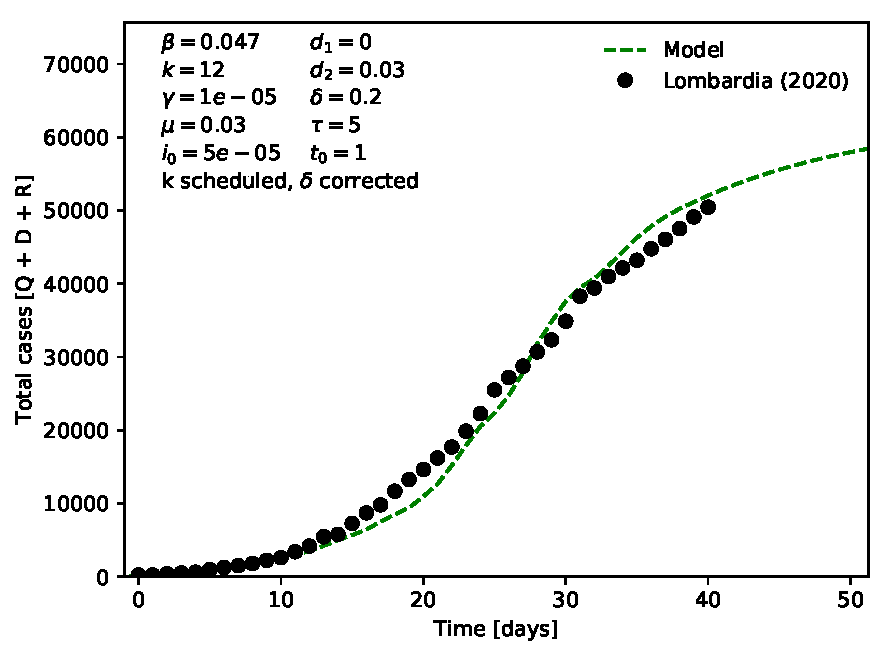
\includegraphics[width=0.4\textwidth]{imgs/Covid/DataVsModel_parameters_Lombardia_scheduling_corrected_definitive.pdf} }
  \caption{Prediction of the improved model for the population classes with the correction with a new set of tuned parameters (a). Comparison of the model in (a) with the data collected in Lombardy (b).}
  
\end{figure}

The two corrections are shown in Figure~\ref{fig:scheduling}. With this new features, a new set parameters have been tuned to approximately match with data shape, the prediction of the tuned mode is shown in Figure~\ref{fig:model_vs_time}, while the comparison with data is presented in Figure~\ref{fig:model_vs_data}.\\


\subsection{Profile likelihood fit to data}
\label{ssec:plf}

The model parameters are here measured in a Profile Likelihood fit. The fit has been performed using \textsc{ROOT} Framework \cite{ROOT} and in particular the \emph{HistFactory} framework to create statistical models \cite{HistFactory}.\\

 The used observable is the number of new total cases (deaths, quarantined and recovered) to get uncorrelated quantities for each bin of the fitted distribution. The distribuition has been rebinned to decrease statistical jumps bin-by-bin. The Parameter of Interest (PoI) is an additional global normalisation factor of the distribution, introduced as a free floating parameter. This corresponds to a variation of the initial condition, $i_0$. The profile likelihood fit adjust the model parameters to maximise the likelihood \cite{HistFactory}.\\
 
 
Since no functional dependence of the model is available, templates of the distribution for different choice of the model parameters are generated and used in the fit. For each parameter of the model, two templates of the distribution are generated, corresponding of increasing and decreasing of a $10\%$ the parameter value. To each of them a Gaussian prior is associated and fitted, with a variance corresponding to the variations described. For middle points, an interpolation is used bin-by-bin, to get the effect of the parameter on the distribution. These parameters are used as Nuisance Parameters (NPs) in the fit, the example for two NPs variations are shown in Figure~\ref{fig:syst_np}. To improve the fit stability the effect of the NPs are symmetrised against the nominal prediction. In case both variations are on one side, as in Figure~\ref{fig:syst_np}b, the variation is one-sided symmetrised. In case of $\mu$ parameter, a higher value increases the number of quarantined per day, while its decrease makes the spreading going faster, increasing the number of infected and then quarantined as well. Therefore, this variation is symmetrised on both sides.\\

\begin{figure}
\centering
\subfloat[]{ 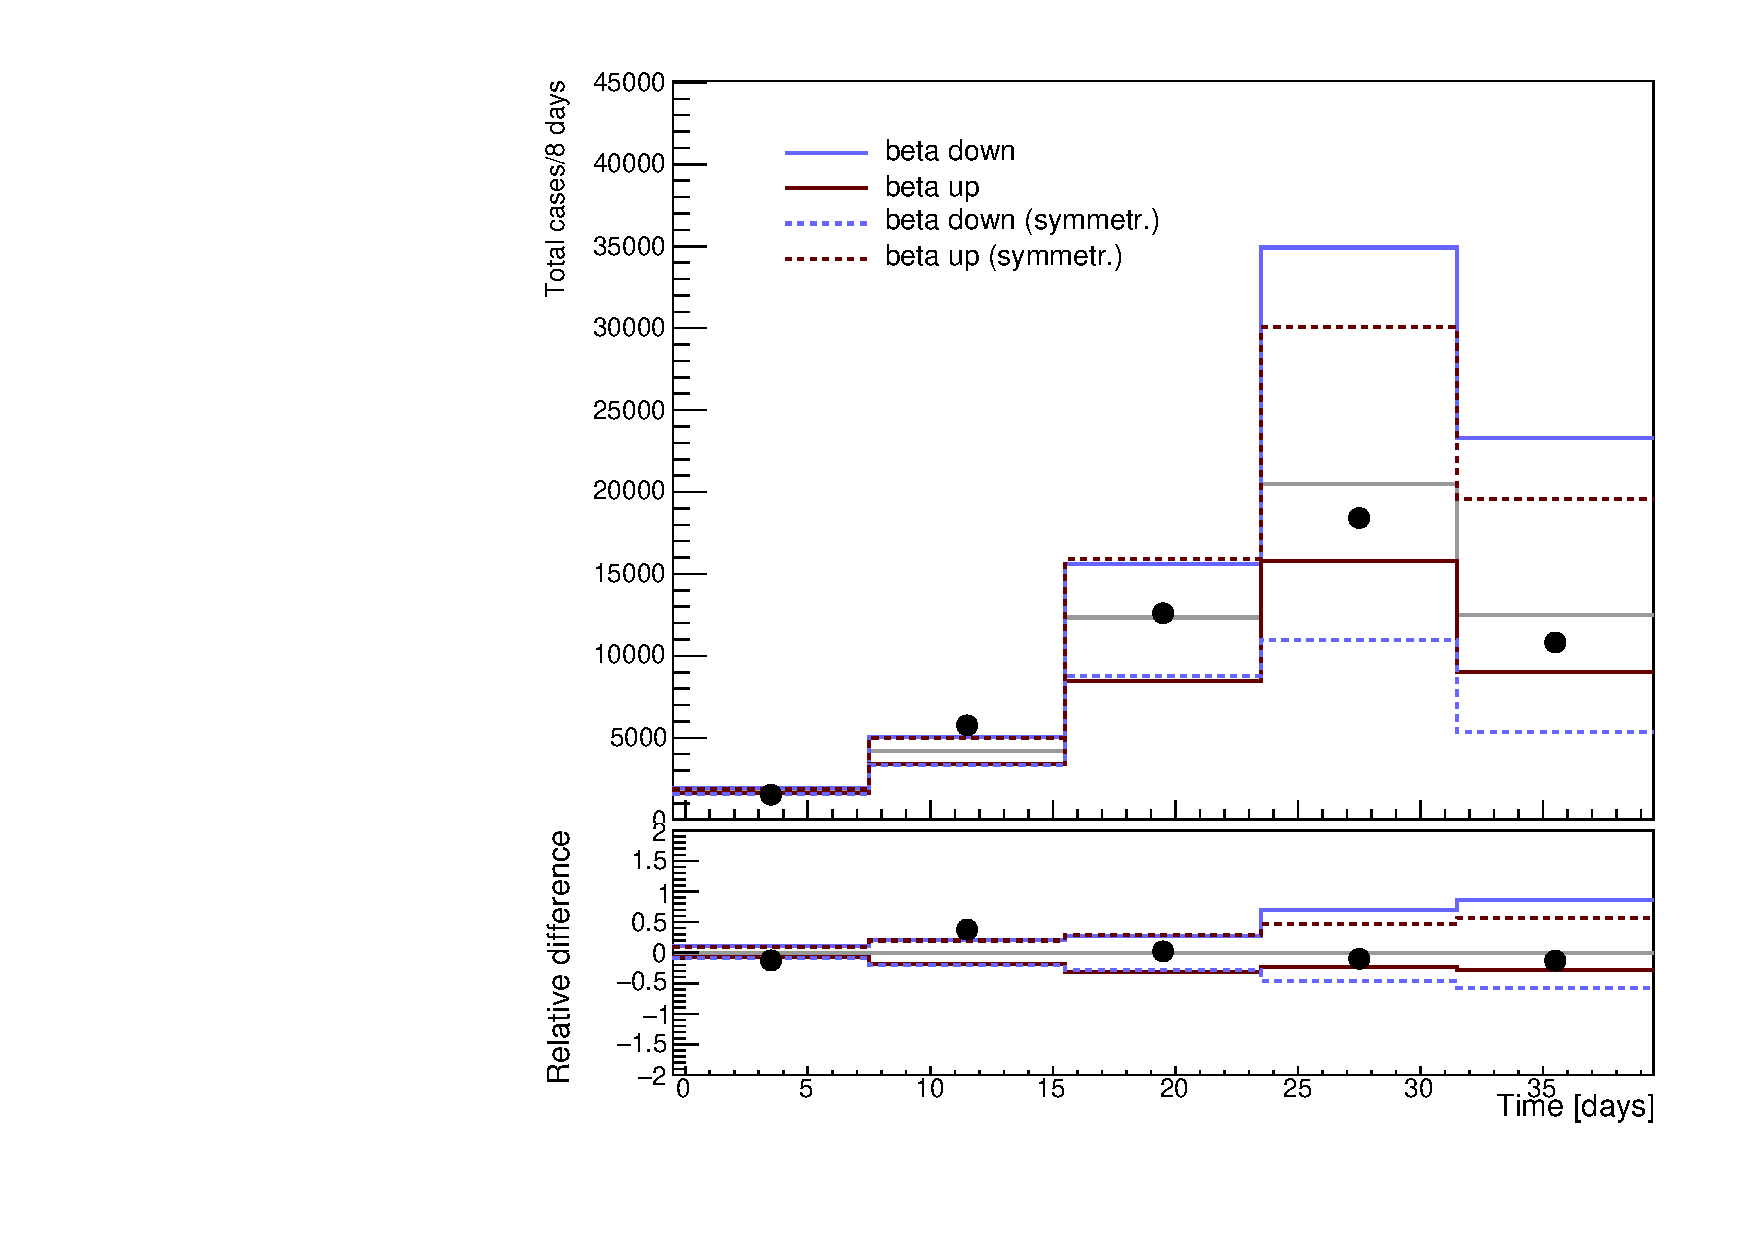
\includegraphics[width=0.4\textwidth]{imgs/Covid/Syst_beta.pdf} }
\subfloat[]{ 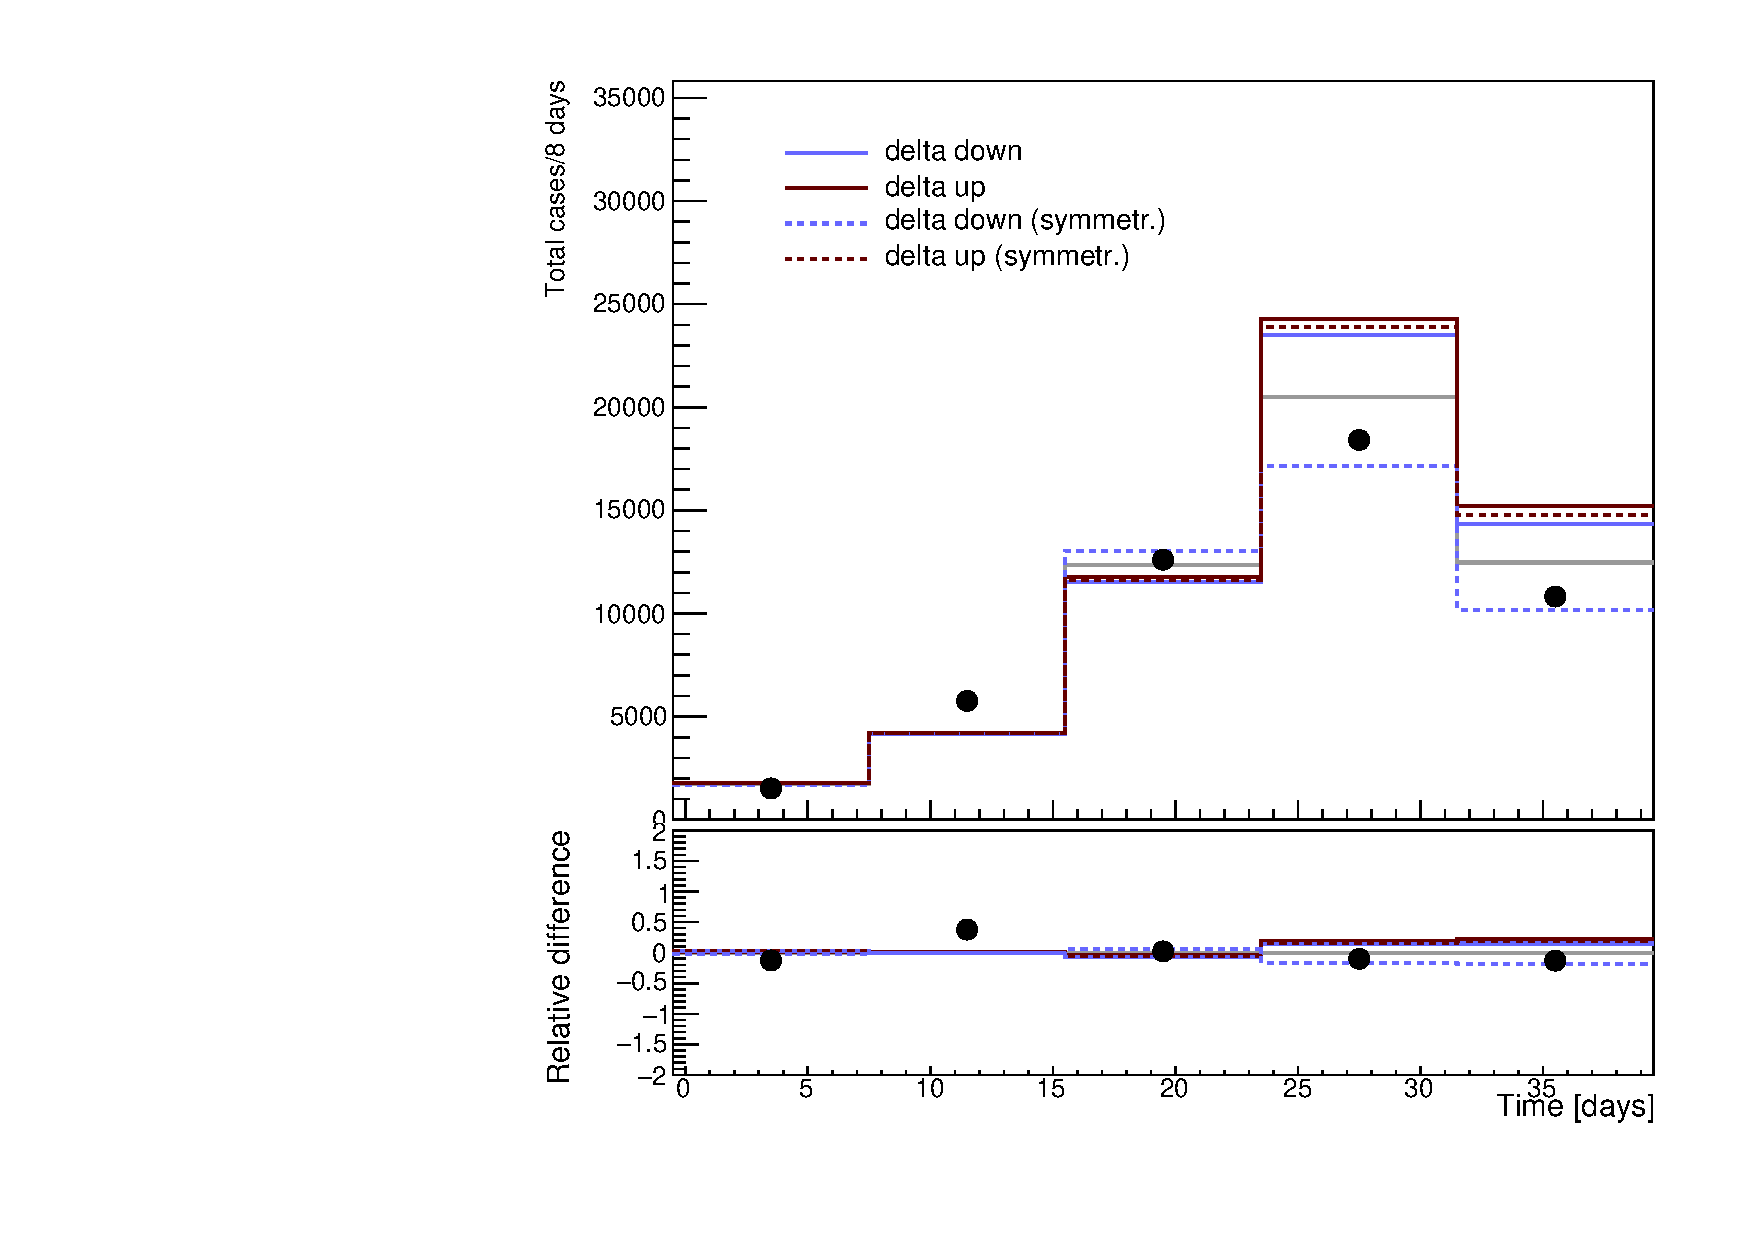
\includegraphics[width=0.4\textwidth]{imgs/Covid/Syst_delta.pdf} }
  \caption{Two examples of NPs included in the fit: variation of $\beta$ (a) and $\mu$ parameters.}
  \label{fig:syst_np}
\end{figure}

To give enough degrees of freedom to the fit, additional NPs are used to take into account uncertainty on the tests-based $\delta$ correction. From Figure~\ref{fig:tests_vs_time} an approximate variance of $20\%$ is estimated, and a NPs for each bin is added, assuming that the variations are uncorrelated bin-by-bin. The example for the two highest bins are shown in Figure~\ref{fig:syst_np_corrbin}.

\begin{figure}
\centering
\subfloat[]{ 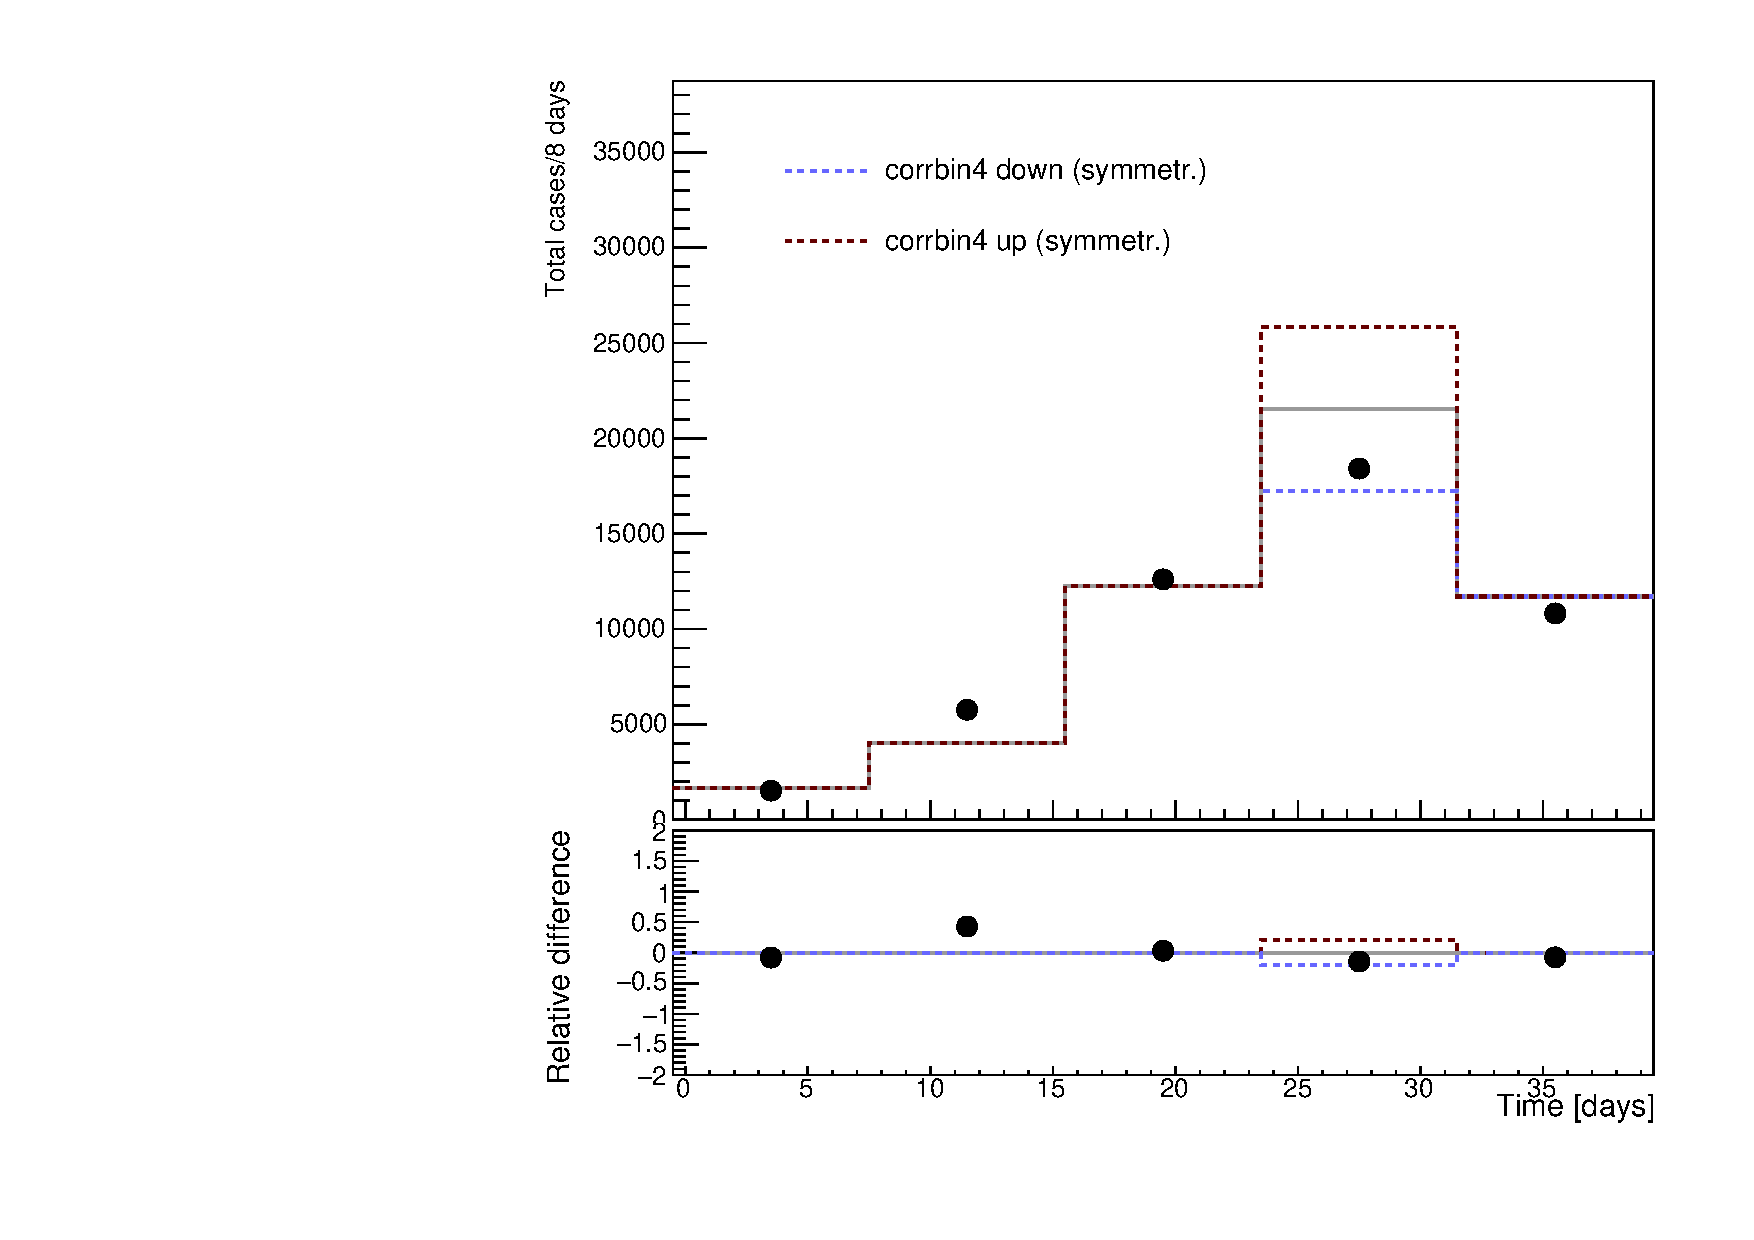
\includegraphics[width=0.4\textwidth]{imgs/Covid/Syst_corrbin4.pdf} }
\subfloat[]{ 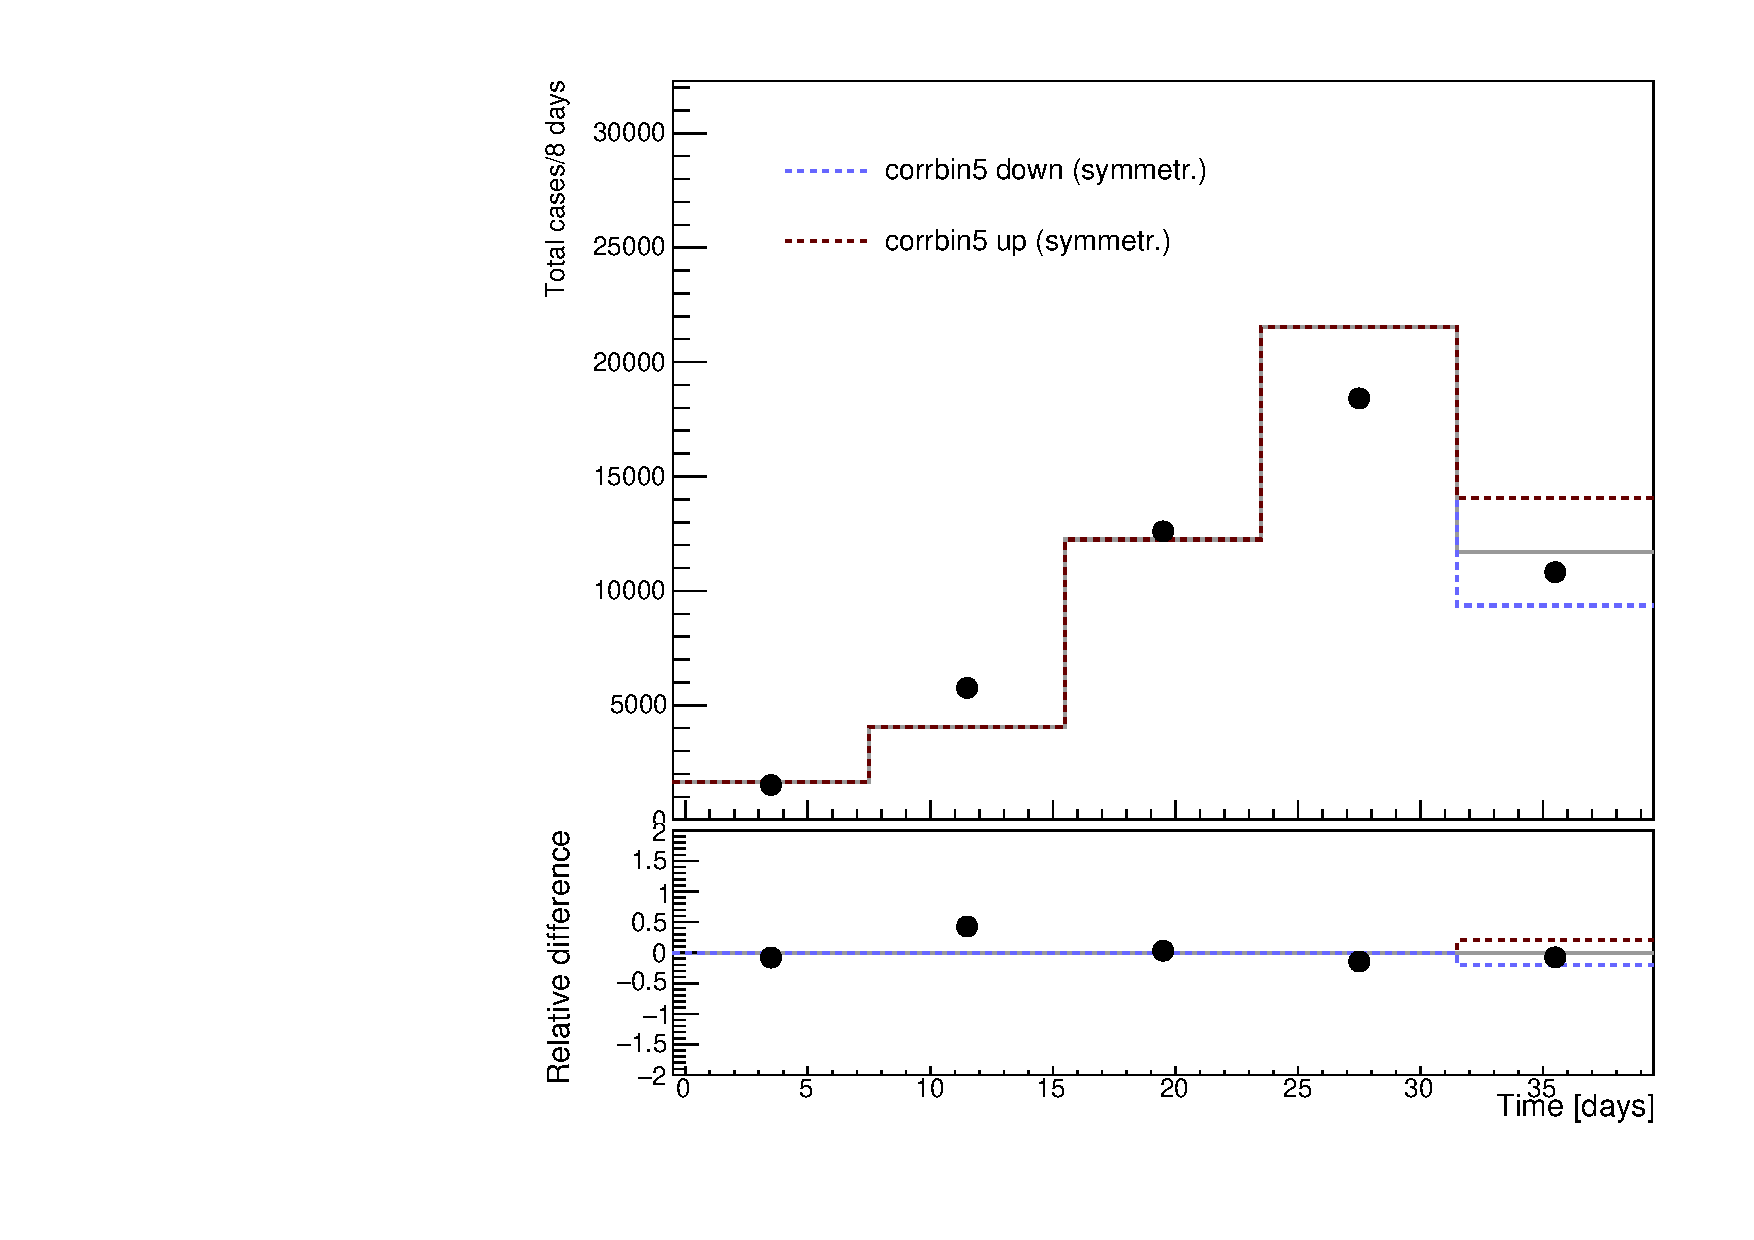
\includegraphics[width=0.4\textwidth]{imgs/Covid/Syst_corrbin5.pdf} }
  \caption{Variations associated to the test-based $\delta$ parameter corrections on the most significant bins in terms of shape of the distribution.}
  \label{fig:syst_np_corrbin}
\end{figure}

The pre-fit prediction is shown in Figure~\ref{fig:prefit}. The summary of the fitted model parameters and their correlations are shown in Figure~\ref{fig:nps}. Figure~\ref{fig:nps}a shows the pre-fit NPs value, equal to zero, following a Normal Gaussian distribution. The points indicate the post-fit values and associated uncertainties. The uncertainties on the parameters are constrained, meaning that the assumed systematics model is conservative and the NPs are measured with a higher precision than the assumptions. Large pulls, over one standard deviations are observed in just two NPs, corresponding to the correcions on the bin contents. This is acceptable since the  uncertainty is estimated by assuming the fluctuation coming from a Gaussian on the fitted model in Figure~\ref{fig:tests_vs_time}. In case the Lombardy tests are way different from the coutry-wise data in some periods, this assumption may be wrong and pulls appear. The parameter of interest, denoted as \emph{SF}, is expected to be unitary and still fitted consistently to be one in one standard deviation. Correlations between parameters are understood: the scale factor, $\beta$, $\tau$ and the bin corrections are the most correlated, since they strongly affect the distribution shapes in different ways, and arranged to counter-balance the effects among themselves. The post-fit prediction is shown in Figure~\ref{fig:postfit}.

\begin{figure}
\centering
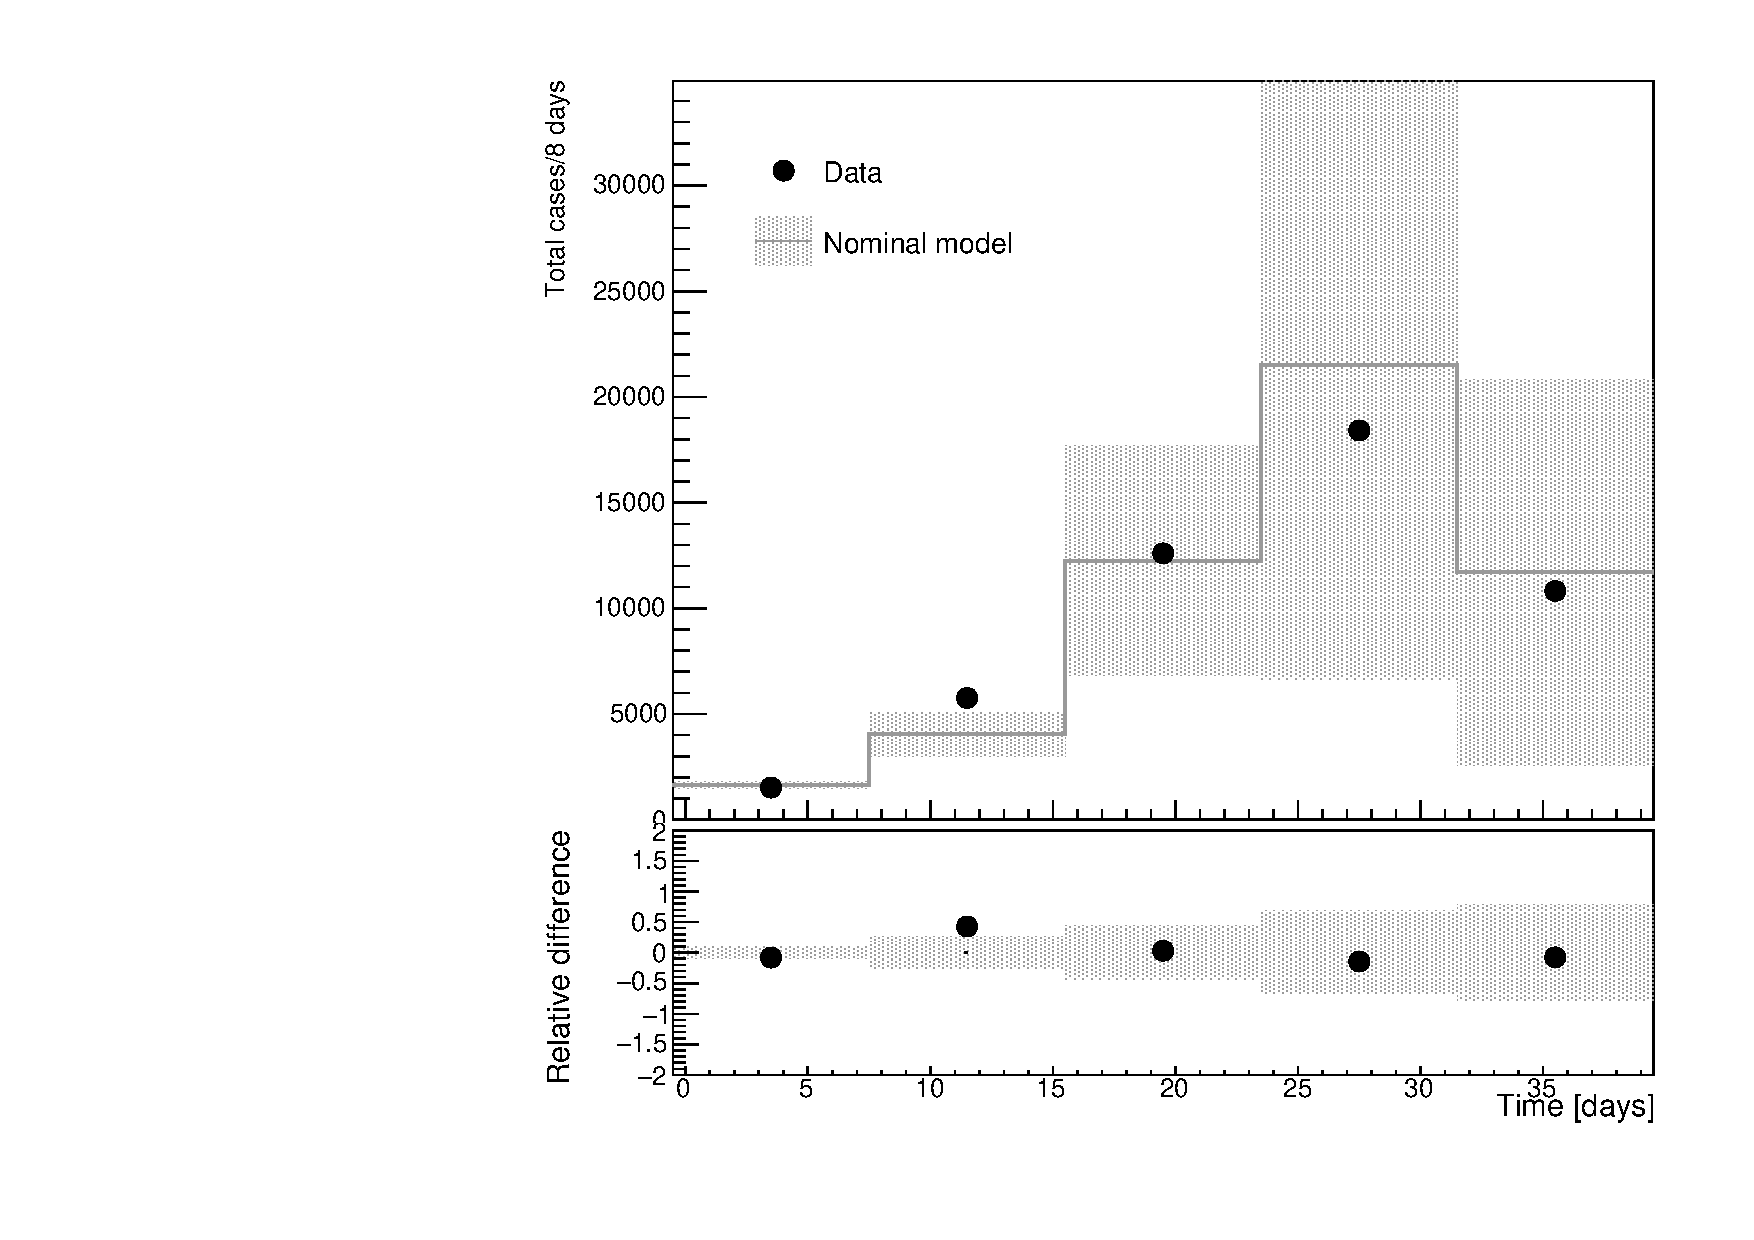
\includegraphics[width=0.4\textwidth]{imgs/Covid/ModelPrefit.pdf} 
  \caption{Pre-fit prediction of the model with the corrections described in Figure~\ref{ssec:impr_model} and the parameters in Figure~\ref{fig:model_vs_time}. The total uncertainty is given by summing all the sources of uncertainties described in Section~\ref{ssec:plf}}
  \label{fig:prefit}
\end{figure}

\begin{figure}
\centering
\subfloat[]{ 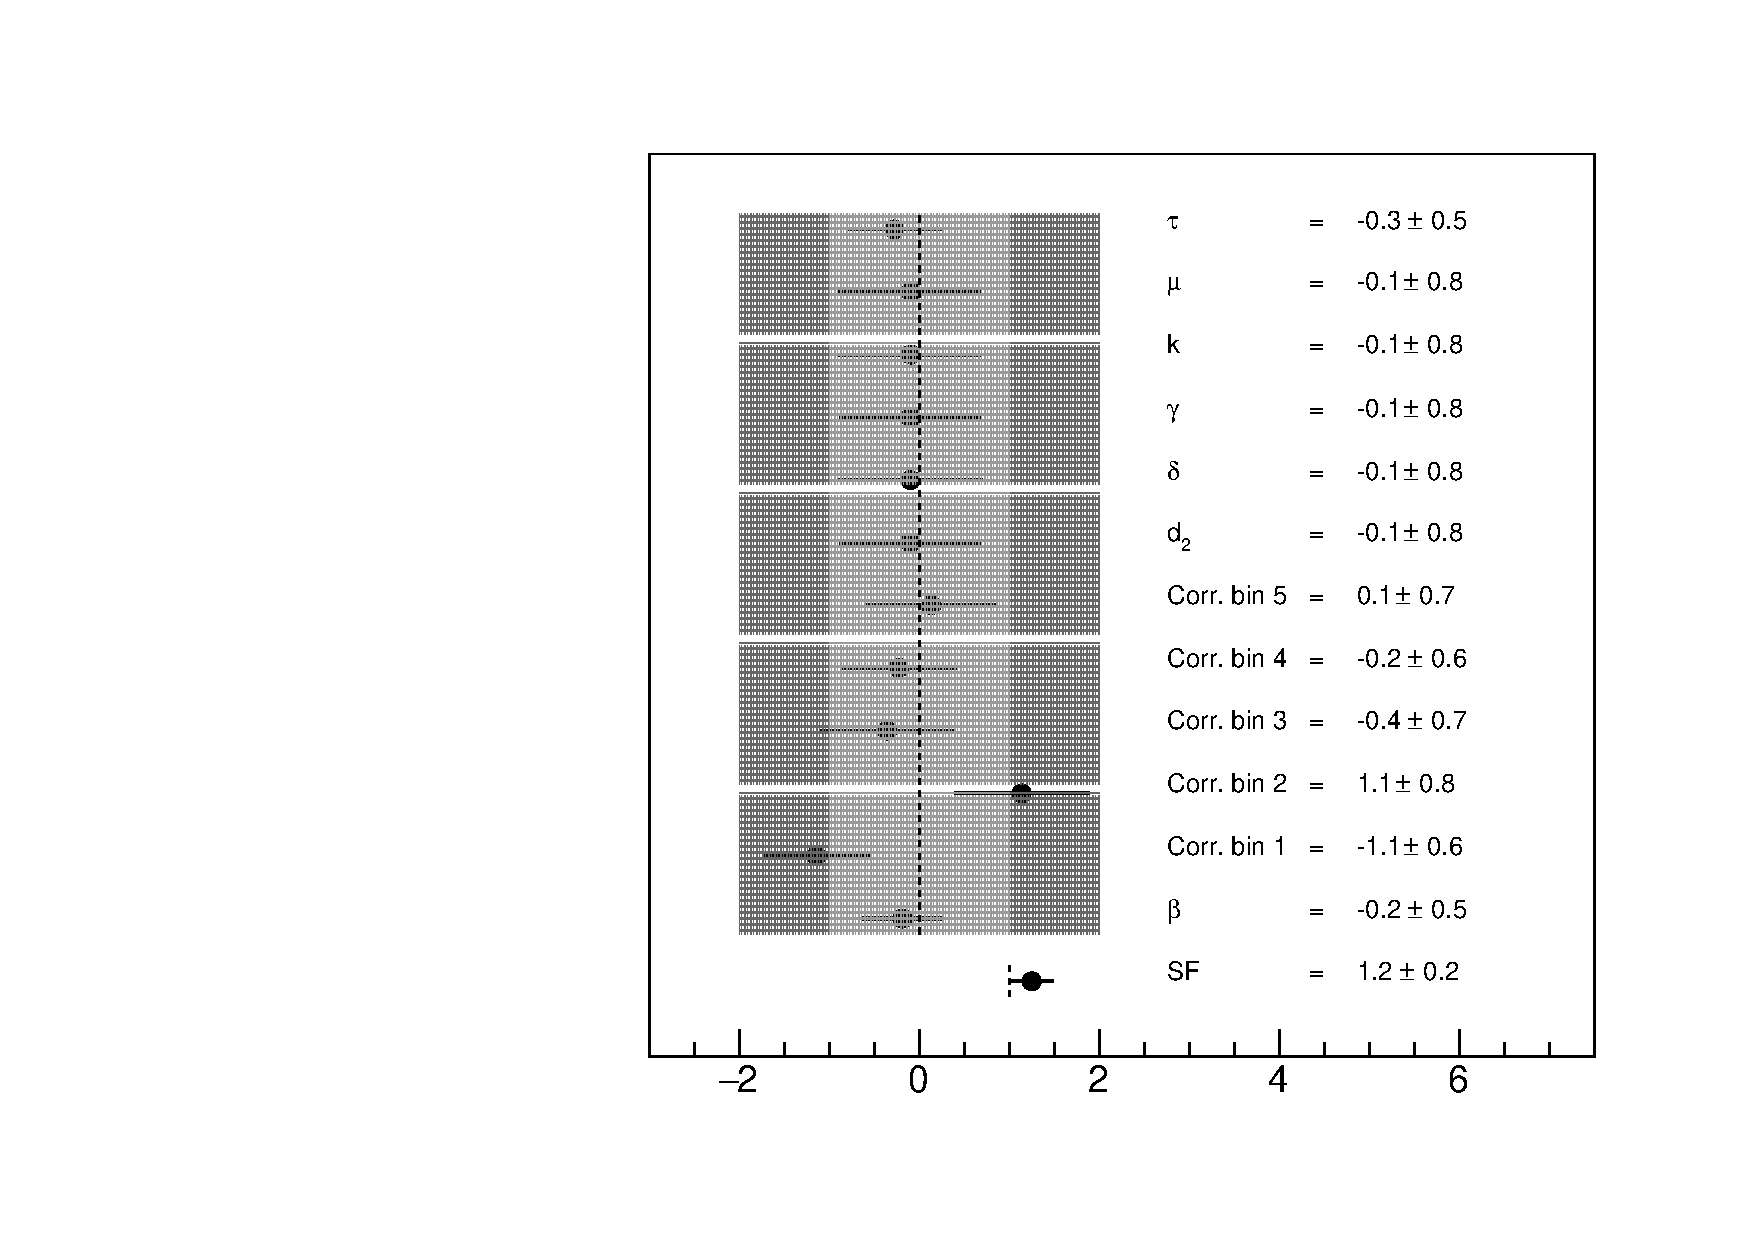
\includegraphics[width=0.45\textwidth]{imgs/Covid/PoI.pdf} }
\subfloat[]{ 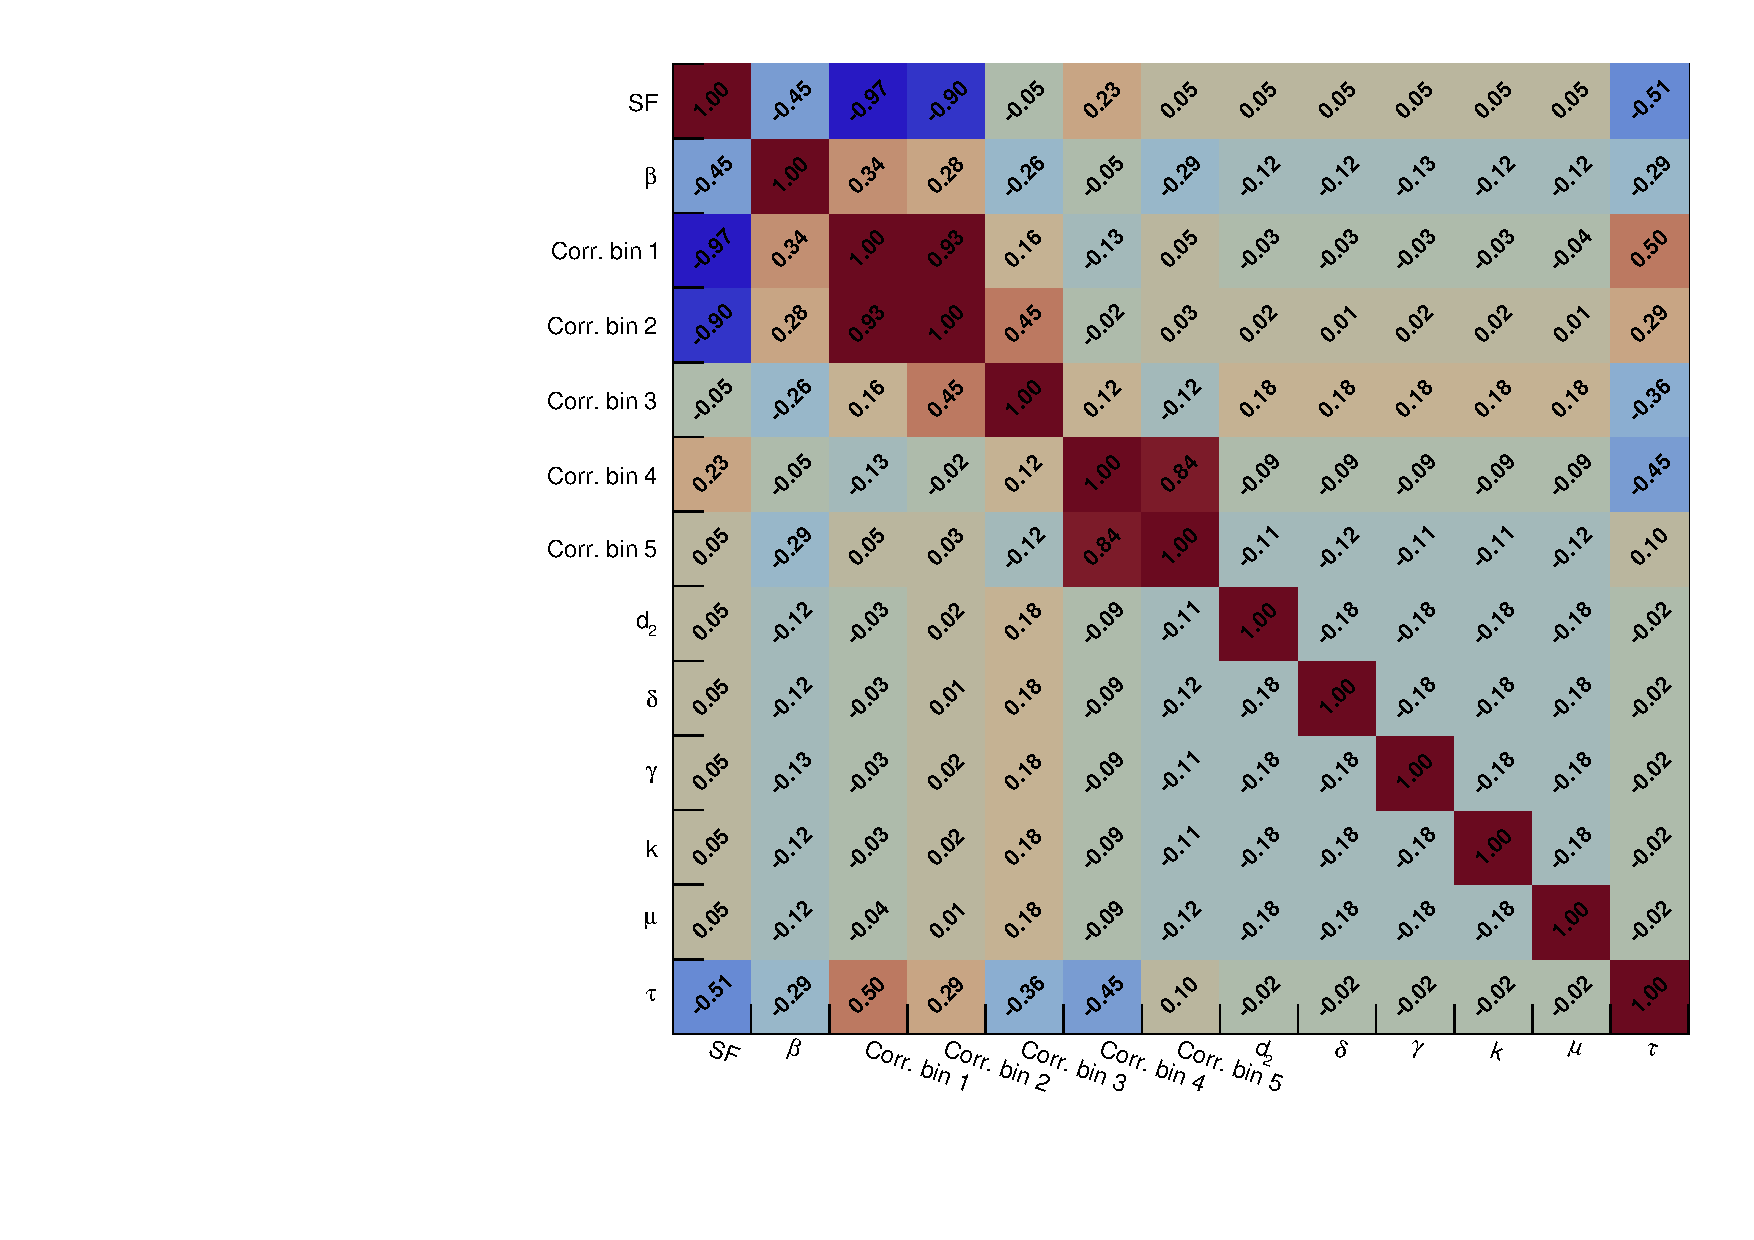
\includegraphics[width=0.4\textwidth]{imgs/Covid/CorrMatrix.pdf} }
  \caption{Fitted values of the model parameters (a). Correlations between the fitted parameters (b).}
  \label{fig:nps}
\end{figure}

The uncertainties are shrinked at higher bins, while enlarged in the lower bins because of the pulls and shows good agreement of the model with data within the fitted uncertainties.

\begin{figure}
\centering
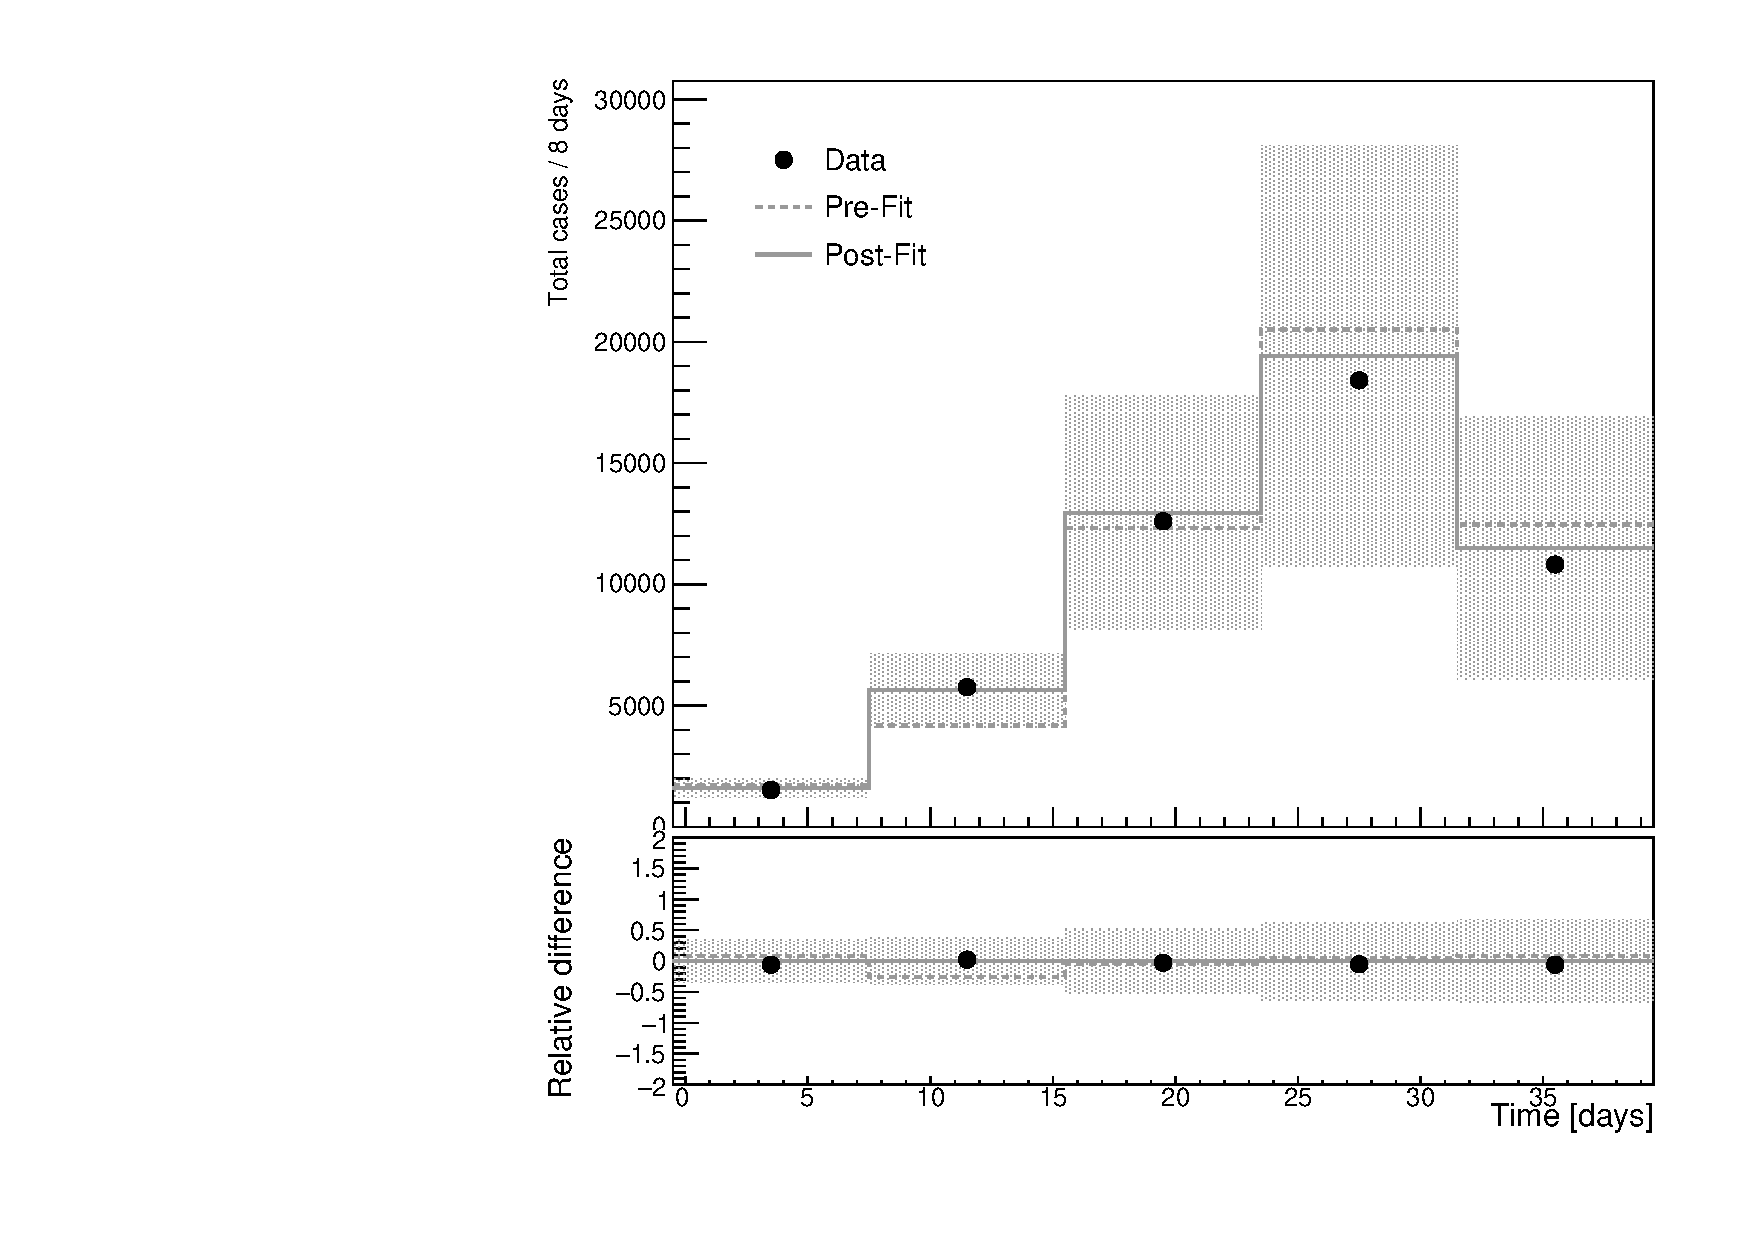
\includegraphics[width=0.4\textwidth]{imgs/Covid/ModelPostFit.pdf} 
  \caption{Post-fit prediction of the model with the corrections described in Figure~\ref{ssec:impr_model}, with parameters pulled as in Figure~\ref{fig:nps}a. The total uncertainty is given by summing all the post-fit uncertainties, correlated as in Figure~\ref{fig:nps}b.}
  \label{fig:postfit}
\end{figure}

\subsection{Predictions}
The fitted set of parameters is used to make a prediction of the population classes evolutions, as shown in Figure~\ref{fig:model_postfit}.

\begin{figure}
\centering
\subfloat {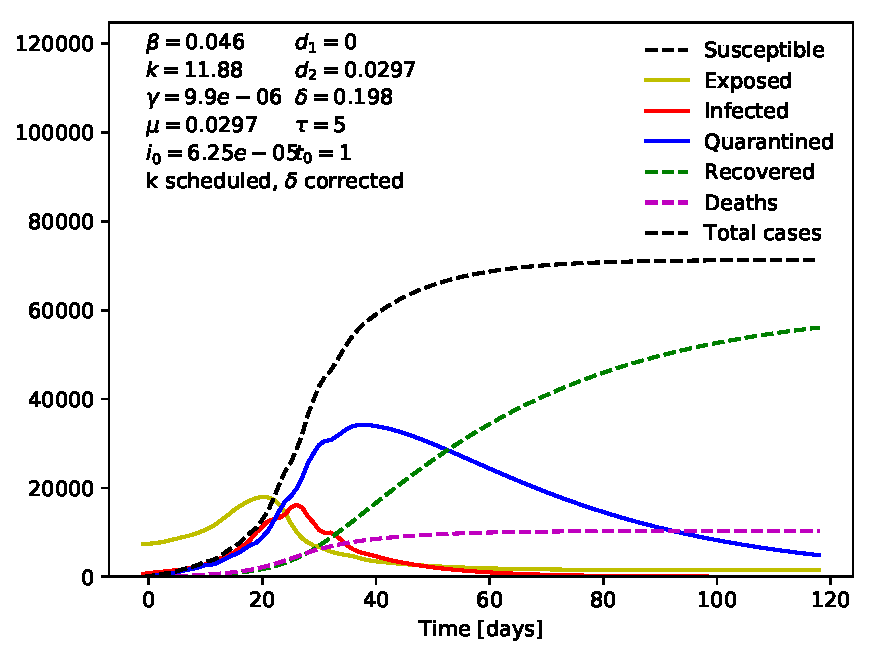
\includegraphics[width=0.4\textwidth]{imgs/Covid/Summary_parameters_Lombardia_scheduling_corrected_postfit.pdf}  }
\subfloat {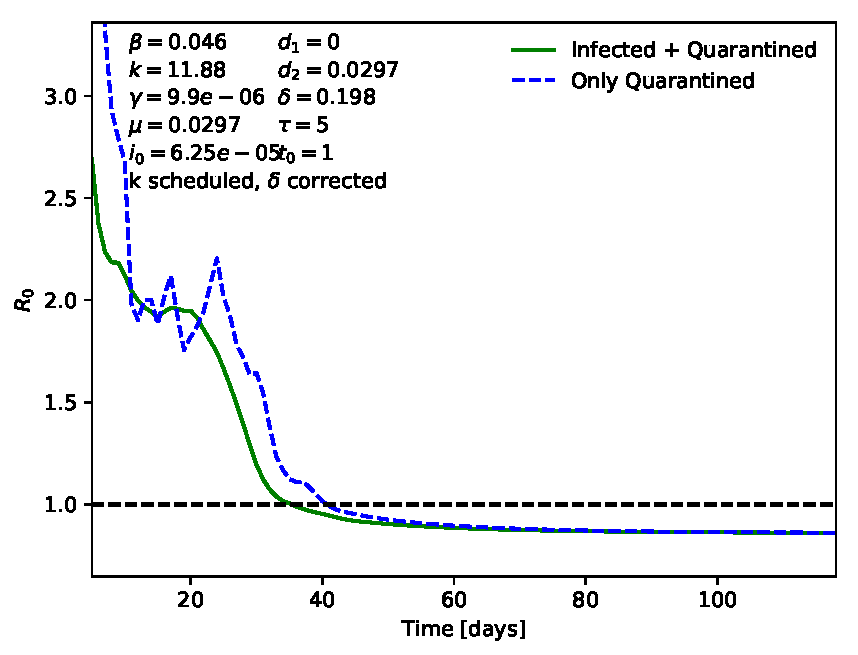
\includegraphics[width=0.4\textwidth]{imgs/Covid/R0_parameters_Lombardia_scheduling_corrected_postfit.pdf}  }
  \caption{Prediction of the model tuned with the fitted parameters in Figure~\ref{fig:nps}a. Prediction of $R_0$ parameter against time (b).}
  \label{fig:model_postfit}
\end{figure}

The model can be used to make some predictions of some observables and test it with observations. To estimate the uncertainty, a set of $1000$ pseudo-experiments is generated, obtained by extracting values of the parameters from the fitted distributions, taking into account the fitted correlations. Predictions are made by estimating mean and variance of the obtained distributions. Since the fit is performed on the total cases distributions, predictions on these quantities are more reliable. However, since quarantined population is the largest, especially in the fitted range, among the contributions in the total cases, also this estimation should be robust. The predictions on the number of number of deaths may be affected by the small contribution in the total case in the fitted range, and therefore not robust. However, in the initial tuning, the ratios between the contributions of the different classes is taken into account, so the obtained numbers should be in the same order of magnitude of the observations. A summary of all the predictions is summarised in Table~\ref{tab:predictions}.

\begin{table}\centering
\begin{tabular}{@{}lll@{}}
\toprule
Quantity & \phantom{abc} & Value \\
\midrule
\multicolumn{3}{@{}l@{}}{\emph{Quarantined people}}\\[1mm]
Peak & \phantom{abc} & $ 36000 \pm 17000 $\\
Peak time & \phantom{abc} & $ 38\pm1 $ days\\[3mm]

\multicolumn{3}{@{}l@{}}{\emph{Deaths}}\\[1mm]
Total deaths & \phantom{abc} & $ 11000 \pm 7000 $\\[3mm]

\multicolumn{3}{@{}l@{}}{\emph{Total cases}}\\[1mm]
Total & \phantom{abc} & $ 77000 \pm 46000 $\\
Saturation time & \phantom{abc} & $ 53\pm6 $ days\\
\bottomrule
\end{tabular}
\caption{Prediction of the model tuned with the fitted parameters in Figure~\ref{fig:nps}a. Dates are expressed in days after February 27th, the first day of available data.}
  \label{tab:predictions}
\end{table}

Currently (on 13/04/2020), from the updated data on \cite{Lab24}, there are $60.314$ total cases, with $10.901$ deaths. Both numbers are compatible with the predictions. The model predicts the peak new quarantined (tested positive) cases on April 2nd, but not a simple comparison with data is possible. The observed peak of total new cases is observed between March 21st and 26th, 2020, one week earlier, but the peak of the daily new cases comes before the peak of quarantined population. A first decrease of total intensive care has been observed on April 5th, close to the expected peak. A comparison in terms of $R_0$ parameter is also possible. This corresponds to the infection power of each single individual. Here it is estimated as ratio of the quarantined and infected (or just quarantined) population at time $t$ with the same quantity at time $t-\tau$, where $\tau $ is the incubation time. The prediction of $R_0$ is shown in Figure~\ref{fig:model_postfit}, giving a $R_0$ estimated below one with only quarantined population data available around the 40th day, so on April 4th. The first indication of a $R_0<1$ in Italy is on April 9th \cite{R0}, still close to the expectations. However both the previous data are available only national-wise and not for Lombardy only, so results may differ a bit. Finally, the estimated on saturation, meaning reaching the $90$ of total cases, is on the 18/04/2020.\\



